% Alard 2007 notes
% by MSSG, Gabriel, Habib, Marcos Lima and Martin, started Aug 2010
% Current: Sept 21, 2010

\documentclass{article}
\RequirePackage{epsfig}

\title{Filling in Details of Alard 2007 MNRAS Paper}

\author{Collective Brazil DES-SL group}

\usepackage{color}
%\usepackage[pdftex]{color,graphicx}

%%%%%%%%%%%%%%%%%%%%%%%%%%%%%%% Some command macros commonly used

%%%%%%%%%%%%%%%%% MSSG's Def'ns
\def\be{\begin{equation}}
\def\ee{\end{equation}}

\def\bea{\begin{eqnarray}}
\def\eea{\end{eqnarray}}

\def\eqref{eq.(\ref}
\def\figref{Fig.\ref}

\def\prtl{\partial}

\newcommand{\eps}{\epsilon}

\newcommand{\rp}{\right)}
\newcommand{\lp}{\left(}

\newcommand{\rb}{\right]}
\newcommand{\lb}{\left[}

\def\pfpt{ {\prtl f_0 \over \prtl \theta }}

\def\dfdt{{d \overline{f}_0(\theta) \over d \theta}}

\def\dsqfdt{{d^2 \overline{f}_0(\theta) \over d \theta^2}}

\def\fbar{\overline{f}_1}

\def\rar{\rightarrow}

\def\vecrz{\vec{r}_{0}}

\def\hatr{\hat{r}}
\def\hatth{\hat{\theta}}


%%%%%%%%%%%%%%%%% Habib's Def'ns
\def \eps {\epsilon}
\def \te {\theta}
\def \rre {\frac{r}{r_{\mathrm{E}}}} 
\def \pa {\partial}
\def \prre {\left( \rre\right)}

\def \re {r_{\mathrm{E}}}
\def \al {\alpha}
\def \te {\theta}
\def \tep {\theta_p}
\def \kt {\kappa_2}
\def \scriptf {\mathcal{F}}
\def \scriptg {\mathcal{G}}
\def \pa {\partial}


\newcommand{\ML}[1]{\textcolor{blue}{[#1]}}

%%%%%%%%%%%%%%%%%%% Setting margins
%%%%% Command                              %%%%% Defaults
\setlength{\textwidth}{19 cm}                 % 16.8 cm
\setlength{\textheight}{26 cm}                % 23 cm
\addtolength{\evensidemargin}{-5.2 cm}          % -1.6cm
\addtolength{\oddsidemargin}{-3.7 cm}           % -1.6cm
\addtolength{\topmargin}{-2 cm}               % -2.5cm


%%%%%%%%%%%%%%%%%%%%%%%%%%%%%%%%%%%%%%%%%%%%%%%%%%%%%%%%%


\begin{document}
\maketitle
\section{Intro}

Quick reminder for below: $r_s, y, R_0, r_0$ are in the source plane, while $r, x, \theta$ are in the image plane.

\section{Basic Ideas}
%%%%%%%%%%%%%%%%%%%%%%% MSSG

To get to eq.1 of Alard 2007, use $\vec{r}_s = \vec{r} -
\vec{\alpha}$, where $\vec{r}_s$ is the angular position of the point
source in the source plane (see fig. in Narayan and Bartlemann for
this), $\vec{r} = r \hat{r} $ is the angular position of the point
source in the image plane, and $\vec{\alpha}$ is the deflection angle,
which is equal to the radial gradient of the 2D projected potential
$\phi$, which in cylindrical coordinates is

\be
\nabla_r \phi = {\prtl  \phi \over \prtl r} \hat{r} + {1 \over r} {\prtl  \phi \over \prtl \theta} \hat{\theta}.
\ee

(also, we use $ \hat{r}, \hat{\theta}$ in place of Alard's $\hat{u_r},
\hat{u_\theta}$).

Thus 

\bea
\vec{r}_s & = & r \hat{r} - \lp {\prtl  \phi \over \prtl r} \hat{r} - {1 \over r} {\prtl  \phi \over \prtl \theta} \hat{\theta} \rp \\
\label{eq:rs}
& = & \lp r -  {\prtl  \phi \over \prtl r} \rp \hat{r} -  {1 \over r} {\prtl  \phi \over \prtl \theta} \hat{\theta} 
\eea

Now let's go to the simplest case of an on-axis point source with
perfectly axially symmetric potential $\phi = \phi_0$.  In this case
$r_s = 0, {\prtl \phi_0 \over \prtl \theta} = 0$ since there is no
angular variation of the potential.

Thus, eq.(\ref{eq:rs}) reduces to

\be
0 =  r -  {\prtl  \phi \over \prtl r} 
\ee

or

\be
\label{eq:einsteinradius}
  r =  \left. {\prtl  \phi \over \prtl r} \right|_{r_E} = r_E
\ee

Where the derivative of the potential is to be evaluated at the Einstein radius, $ {r_E}$.

This indicates the point source is spread into a circle of radius $ {r_E}$ in the image plane.

We now take the first step of perturbing the situation:

\bea
\label{eq:rspert}
r_s & = & \eps y \\
\phi & = & \phi_0 + \eps \psi
\eea

which imply we have moved the source off-axis, and added a non-axially
symmetric potential, both to the exact same order $\eps$ by
assumption.  Note that the perturbed distance $y$ is in the source plane.

Note that this changes the notation of the first eq in Alard eq.3
(which is fairly nonsensical, of course).

Eq.(\ref{eq:rspert}) leads to a modification of eq.(\ref{eq:einsteinradius}) into

\be
\label{eq:rpert}
r = r_E + \eps x
\ee

which changes the notation in Alard eq.4 (which is somewhat weird
notation, since his $dr$ is not necessarily a small distance), and we
do not follow his convention of setting $r_E \equiv 1$.
  
Note that now the perturbed distance $x$ is in the image plane.

To recap: $r_s, y$ are in the source plane, while $r, x$ are in the image plane.

Now we do a Taylor series expansion of the potential:

\be
\phi = \phi_0 + \eps \psi = \sum_{n=0}^\infty {1 \over n!} \left. {d^n \phi_0 \over dr^n }\right|_{r_E} (r-r_E)^n + \eps {1 \over n!} \left. {d^n \psi(\theta) \over dr^n }\right|_{r_E} (r-r_E)^n 
\ee

or

\be
\label{eq:tse}
\phi  = \sum_{n=0}^\infty \left[ {1 \over n!} \left. {d^n \phi_0 \over dr^n }\right|_{r_E} + \eps {1 \over n!} \left. {d^n \psi(\theta) \over dr^n }\right|_{r_E} \right] (r-r_E)^n 
\ee

And now define

\be
C_n \equiv {1 \over n!} \left. {d^n \phi_0 \over dr^n }\right|_{r_E} 
\ee

\be
f_n(\theta) \equiv  {1 \over n!} \left. {d^n \psi(\theta) \over dr^n }\right|_{r_E}
\ee

So that we can write  eq.(\ref{eq:tse}) as

\be
\label{eq:tse2}
\phi  = \sum_{n=0}^\infty \left[ C_n + \eps f_n  \right] (r-r_E)^n 
\ee

where $f_n = f_n(\theta)$.

Now let's go back and substitute \eqref{eq:rspert}) and \eqref{eq:rpert}) into \eqref{eq:rs}) to find

\be
\eps y = \lp r_E + \eps x -  {\prtl  \phi \over \prtl r} \rp \hat{r} - {1 \over r_E + \eps x}  {\prtl  \phi \over \prtl \theta} \hat{\theta} 
\ee

Now substitute \eqref{eq:tse2}) into this to find

\bea
\eps y = \lp r_E + \eps x -  {\prtl \over \prtl r} \lp \sum_{n=0}^\infty \left[ C_n + \eps f_n  \right] (r-r_E)^n  \rp \rp \hat{r} - \\
{1 \over r_E + \eps x}  {\prtl  \over \prtl \theta} \lp \sum_{n=0}^\infty \left[ C_n + \eps f_n  \right] (r-r_E)^n  \rp  \hat{\theta} \nonumber
\eea

Remembering that $C_n, f_n$ are independent of $r$, and using $r-r_E = \eps x$ :
 
\bea
\label{eq:tse3}
\eps y = \lp r_E + \eps x -   \sum_{n=0}^\infty \left[ C_n + \eps f_n  \right] n (\eps x)^{n-1}  \rp \hat{r} - \\
{1 \over r_E + \eps x}  {\prtl  \over \prtl \theta} \lp \sum_{n=0}^\infty \left[ C_n + \eps f_n  \right] (\eps x)^n  \rp  \hat{\theta} \nonumber
\eea


Let us expand \eqref{eq:tse3}) in orders, first the zero'th order piece in $\eps$:


\be
0 =  \lp r_E  -C_1 \rp \hat{r} \rightarrow r_E = C_1 = \left. \prtl \phi \over \prtl \theta \right|_{r_E}
\ee


Next the first order piece in $\eps$:


\be
\eps y = \lp \eps x - (2 C_2 \eps x + \eps f_1 ) \rp \hat{r} - {1 \over r_E} \eps {\prtl f_0 \over \prtl \theta } \hat{\theta}
\ee

where the coefficient of $C_2$ was expanded to order with $n=2$, that of the $f_1$ term with $n=1$, and that of the $\prtl f_1 \over \prtl \theta$ term with $n=0$.  Bit involved, but this is how to get each term proportional to $\eps$.

Now divide through by $\eps$ and collect terms:

\be
 y = \left[ (1-2 C_2) x -  f_1 \right] \hat{r} - {1 \over r_E} \pfpt  \hat{\theta}
\ee

or, defining $\kappa_2 = 1-2 C_2$

\be
\label{eq:rsexpanded}
 y = \left[ \kappa_2  x - f_1 \right] \hat{r} - {1 \over r_E}  \pfpt  \hat{\theta}
\ee

which is Alard eq.8 (remember he set $r_E \equiv 1$).


\section{Reconstruction of Images}

%%%%%%%%%%%%%%%%%%%%%%%%%%%%%%%%%%%%%%%%%%%%%%%%%%%%%%%%%%%%%%%%%%%%%%%%%%%%%%%%%%%%%%%%%%%%%%%%%%%%%%%%%%%%%%%%%%%%%%%%%%%%%%%
%%%%%%%%%%%%%%%%%%%%%%%%%%%%%%%%%%%%%%%%%%%%%%%%%%%%%%%%%%%%%%%%%%%%%%%%%%%%%%%%%%%%%%%%%%%%%%%%%%%%%%%%%%%%%%%%%%%%%%%%%%%%%%%
%%%%%%%%%%%%%%%%%%%%%%%%%%%%%%%%%%%%%%%%%%%%%%%%%%%%%%%%%%%%%%%%%%%%%%%%%%%%%%%%%%%%%%%%%%%%%%%%%%%%%%%%%%%%%%%%%%%%%%%%%%%%%%%

\subsection{Circular Source Contours}
%%%%%%%%%%%%%%%%%%% Gabriel

In this section we study the mapping of a circular contour using this formalism.

Notation: $ \vec{r}_{0}$ points from the origin (i.e center of the
source plane, looking directly on-axis from us through the lens to the
source) to the center of the actual source object (like a small
circular galaxy), $ \vec{R}_{0}$ is the vectorial radius of this
source from its center, and $ \vec{r}_{s}$ is the vector from the
origin to some point on the edge of the circular source. As a first
stab, see \figref{fig:sourceplane} for this configuration.



\begin{figure}
\begin{center}
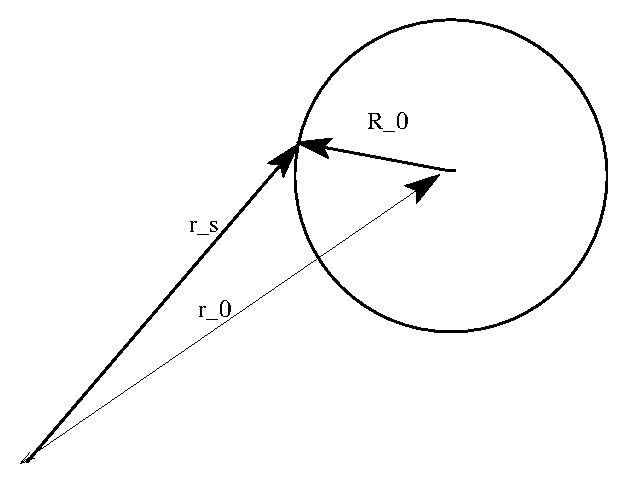
\epsfig{file=sourceplane.eps,height=4.8cm,angle=0}
\caption{\label{fig:sourceplane} Circular source in the source plane.}
\end{center}
\end{figure}

So:

\be
\vec{r}_s =  \vec{r}_{0} + \vec{R}_{0} , \;\;\; \rar \vec{R}_{0} = \vec{r}_s - \vec{r}_{0}, \;\;\; 
\ee


Replacing $r_s$ by \eqref{eq:rsexpanded}), we obtain:

\be
\label{eq:Rzero}
\vec{R_{0}} = \left[ \kappa_2 x - f_{1}(\theta) \right]\hat{r} - \frac{1}{r_E} \frac{\partial f_0(\theta)}{\partial \theta} \hat{\theta} - \vec{r_{0}}. \;\;\; 
\ee


Note that $\vec{r}_{0} = (x_0,y_0)$ lies in the source plane, but we
can write it in terms of the polar unit vectors 

\bea
\label{eq:unitvs}
\hat{r}=(\cos\te, \sin \te) \\
\hat{\theta}=(-\sin \te, \cos \te)
\eea

 as following

\be
\vecrz = (\vecrz \cdot \hatth) \hatth + (\vecrz \cdot \hatr) \hatr
\ee

or

\be
\label{eq:rzero}
\vec{r}_{0} = \lb x_0 \,  \cos \te + y_0 \,  \sin \te \rb \hat{r} + \lb -x_0 \,  \sin \te + y_0 \,  \cos \te \rb \hat{\theta}.  \;\;\; 
\ee

So that \eqref{eq:Rzero}) becomes

\be
\vec{R_{0}} = \left[ \kappa_2 x - f_{1}(\theta) \right]\hat{r} - \frac{1}{r_E} \frac{\partial f_0(\theta)}{\partial \theta} \hat{\theta} -  \lb x_0 \,  \cos \te + y_0 \,  \sin \te \rb \hat{r} + \lb -x_0 \,  \sin \te + y_0 \,  \cos \te \rb \hat{\theta} \;\;\; 
\ee

Defining 

\be
\overline{f}_i(\theta) = f_i(\theta) + (x_0 \cos \te + y_0 \sin \te)r_{E}^{1-i}, \;\; i=0,1
\ee

this becomes

\be
\vec{R}_{0} = \left[ \kappa_2 x - \overline{f}_{1}(\theta) \right]\hat{r} - \frac{1}{r_E} \frac{\partial \overline{f}_0(\theta)}{\partial \theta} \hat{\theta}. \;\;\; 
\ee

(Alard eq.11).

Now, taking the square of this we obtain

\be
R_{0}^2 = \left[ \kappa_2 x - \overline{f}_{1}(\theta) \right]^2 + \left[\frac{1}{r_E} \frac{\partial \overline{f}_0(\theta)}{\partial \theta}\right]^2. \;\;\; 
\ee

Solving this for $x(\te)$, the radius of the arc in the image plane as
a function of theta, the following two solutions are obtained:

\be
\label{eq:xsoln}
x = \frac{1}{\kappa_2}\left[ \overline{f}_{1}(\theta) \pm \sqrt{R_0^2 - \left( \frac{1}{r_E}\frac{\partial \overline{f}_0(\theta)}{\partial \theta} \right)^2} \right]. \;\;\; 
\ee

corresponding to the inner and outer edges of the arc.

Thus, given the source radius $R_{0}$ and position $(x_0,y_0)$ we can
draw the arcs using \eqref{eq:xsoln}) by varying $\theta$ between
$[0,2\pi[$ and taking the corresponding $x$.


\subsection{Elliptical Source Contours}
%%%%%%%%%%%%%%%%%%% Gabriel

We now extend the discussion of previous section to elliptical contours.

First we can consider the equation of an elliptical contour aligned to
the main axis (note that this is a very limited set of ellipses),

\be
\label{eq:ellipse}
(1-\eta)x_s^2 + (1+\eta)y_s^2 = R_{0}^2.\;\;\; 
\ee

% Use again To write \eqref{eq:rzero} in Cartesian coordinates we use the following relation of the unit vectors:

%\be
%\left\{ \begin{array}{cc} \hat{u}_r = \cos \te\hat{x} + \sin \te\hat{y} \\ \hat{u}_\theta = -\sin \te\hat{x} + \cos \te\hat{y}  \end{array} \right.
%\ee

Now, using \eqref{eq:ellipse})and \eqref{eq:unitvs}) (considering the sources at origin), defining $S = 1-\eta \cos(2\theta)$ and after some algebra we have: (boring according to Gabriel :-) )

\be
x = \frac{1}{\kappa_2} \left\{f_{1}(\theta) + \frac{\eta\sin(2\theta)}{S \, r_E}\frac{\partial f_0(\theta)}{\partial \theta} \pm \frac{1}{S}\sqrt{SR_{0}^2 - (1-\eta^2)\left[ \frac{1}{r_E}\frac{\partial f_0(\theta)}{\partial \theta}\right]^2}  \right\}. \;\;\; (8)
\ee

(Alard eq.15).



\subsection{Conditions for the Validity of the Approximation}
%%%%%%%%%%%%%%%%%%%%%%%%%%%%%%% Habib

At first order in $\eps$ we may define  

\begin{equation}
 q \equiv \frac{r}{r_{\mathrm{E}}}[1-\eps\,g(\te)].
\end{equation}

As the functional $\phi_0(q)$ represents the general expression 
for the perturbed potential, with $q$ defined above, we may expand $\phi_0(q)$

\begin{displaymath}
 \phi_0(q)=\phi_0\left(\rre-\eps\rre\,g(\te)\right)
\end{displaymath}

\noindent in a Taylor Series around $\eps=0$, in the following way

\def\dpdq{ \left. \left( \frac{d\phi_0}{dq}\right) \right|_{\eps=0} }
\def\dpde{ \left. \left( \frac{d\phi_0}{d\eps}\right) \right|_{\eps=0} }

\begin{eqnarray}
 \phi_0(q) &\approx& \phi_0\prre+\eps \dpde \\
	  & = & \phi\prre+\eps \dpdq  \left(\frac{\pa q}{\pa \eps}\right)\\
	  &\approx& \phi\prre-\rre\phi_0^\prime\prre g(\te)\eps \label{key1}
\end{eqnarray}

Where we have defined $\phi_0^\prime\prre \equiv  \dpdq$.  Note, that we have $\phi_0(q)=\phi_0\prre$ when $\eps=0$ and similarly with its derivatives. Therefore,
taking the partial derivatives of Eq.~(\ref{key1}), it is straightforward to verify

\begin{eqnarray}
 r_{\mathrm{E}}\frac{\pa \phi}{\pa r}&=& \phi_0^\prime\prre -%
  \eps\left[g(\te)\phi_0^\prime\prre+\rre g(\te)\phi_0^{\prime \prime}\prre\right]\\
\frac{r_{\mathrm{E}}}{r}\frac{\pa \phi}{\pa \te}&=&-\phi_0^\prime\prre \frac{dg(\te)}{d\te}\eps
\end{eqnarray}

(Alard eq.19).


\subsubsection{Errors on arcs}
%%%%%%%%%%%%%%%%%%%%%%%%%%%%%%% Marcos

Recall that $\phi=\phi_0+\eps\psi$ and expand only $\psi$:

\bea
\phi=\phi_0+\eps\sum_{n=0}^{\infty}f_n(\theta)(r-r_E)^n
\eea

Differentiating we obtain

\bea
\frac{\partial \phi}{\partial r }&=&\phi_0^\prime+\eps\sum_{n=1}^{\infty}f_n(\theta)n(r-r_E)^{n-1} \\
\frac{\partial \phi}{\partial \theta}&=&\eps\sum_{n=0}^{\infty} \frac{\partial f_n}{\partial \theta}(r-r_E)^n
\eea

Evaluating at the Einstein radius $r=r_{\mathrm{E}}$, we have

\bea
\frac{\partial \phi}{\partial r }&=&\phi_0^\prime+f_1(\theta) \\
\frac{\partial \phi}{\partial \theta}&=&\eps \frac{\partial f_0}{\partial \theta}
\eea

On the other hand, evaluating Eqs. 19 in Alard at $r=r_E$, and using Eq. 16 in Alard $\phi_0^\prime=1+2C_2(r-r_{\mathrm{E}}+...$ 

\bea
\frac{\pa \phi}{\pa r}&=& \phi_0^\prime -%
  \eps g(\te)\left[\phi_0^\prime+ \phi_0^{\prime \prime}\right]=\phi_0^\prime-\eps g(\te)(1+C_2)\\
\frac{\pa \phi}{\pa \te}&=&-\eps\phi_0^\prime \frac{dg(\te)}{d\te}
\eea

Comparing these equations, we have a relation between the $f_n(\te)$ and $g(\te)$ functions:

\bea
f_1&=&-(1+2C_2)g \\
\frac{df_0}{d\theta}&=&-\frac{dg}{d\theta}
\eea

Eq. (30) in Alard (to be derived later) is

\bea
dr=\frac{1}{\kappa_2}\left[ f_1+\frac{d^2f_0}{d\theta^2} \right]
\eea

and in this case we have

\bea
dr=\frac{1}{\kappa_2}\left[ -(1+2C_2)g+\frac{d^2g}{d\theta^2} \right]
\eea

Not sure what the effective parameter $dr_c$  in Eq 22 is and how to get it.
Assuming it's correct, i.e.
\bea
dr_c\sim -\frac{d^2g}{d\te^2}-2g
\eea
we have that for e.g. the NFW profile with ellipticity (as in Eq. 28 of Alard)

\bea
\phi_0(q)&=&\frac{1}{2}\log^2\left(\frac{q}{2}\right)-2\arctan^2\left(\sqrt{\frac{1-q}{1+q}}\right) \\
q&=&u_0r\sqrt{1-\eta\cos(\theta)}\approx u_0 r \left[1-\frac{\eta}{2}\cos(2\theta)\right]
\eea

So in this case we have (notice $\eta/2$ plays the role of $\eps$ here, so only expect expansion to work 
for small ellipticities)

\bea
g(\te)&=&\frac{\eta}{2}\cos(2\theta) \\
\frac{d^2g(\te)}{d\te^2}&=&-2\eta\cos(\theta)=-4g
\eea

so that $dr_c=\eta\cos(\theta)$. Not sure if this is true for any elliptical potential or if it's specific to NFW.
In any case the deviation is maximum for $\te=0,\pi$

If the Taylor expansion converges, truncating it at some order has a maximum error given by the next order 
term. In this case the maximum error due to the non-linearity of the gradient of the potential is 

\bea
D=3C_3\max[dr_c^2]=3C_3\eta^2
\eea

Notice it increases with the ellipticity squared. For a general potential of the form

\bea
\phi=\frac{1}{\alpha}r^{\alpha[1+\beta(r-1)]}
\eea

we have

\bea
C_3=\frac{d^3\phi}{dr^3}|_{r=1}=-\frac{(\alpha-1)}{6}+\frac{\beta}{2}
\eea

and $D^2$ follows. 

\subsection{Numerical Testing}

\subsection{Comparison with Ray Tracing}

\subsection{Inverse Modelling}
%%%%%%%%%%%%%%%% MSSG

We'll skip to here, for now.

To get Alard eq.29, take Alard eq. 12:


\be
x = \frac{1}{\kappa_2}\left[ \overline{f}_{1}(\theta) \pm \sqrt{R_0^2 - \left( \frac{1}{r_E}\frac{\partial \overline{f}_0(\theta)}{\partial \theta} \right)^2} \right]. \;\;\; 
\ee

And separate the two solutions for the inner and outer edge of the arc:



\bea
x_i = \frac{1}{\kappa_2}\left[ \overline{f}_{1}(\theta) - \sqrt{R_0^2 - \left( \frac{1}{r_E}\frac{\partial \overline{f}_0(\theta)}{\partial \theta} \right)^2} \right]. \;\;\;  \\
x_o = \frac{1}{\kappa_2}\left[ \overline{f}_{1}(\theta) + \sqrt{R_0^2 - \left( \frac{1}{r_E}\frac{\partial \overline{f}_0(\theta)}{\partial \theta} \right)^2} \right]. \;\;\;  
\eea


Take 

\be
x_o + x_i = {2 \over \kappa_2} \fbar 
\ee

And solve for $\fbar$:


\be
\fbar = {\kappa_2 \over 2} (x_o+x_i)
\ee

which is exactly Alard eq. 29a, without his additional constant (whose provenance I don't get at the moment).

Now take 

\be
x_o - x_i = {1 \over \kappa_2} \lp 2 \sqrt{R_0^2 - {\lp {1 \over r_E} \dfdt \rp}^2 }\rp
\ee

And solve for $\dfdt$ (few straight steps of algebra here):

\be
\dfdt = r_E \sqrt{R_0^2 - {\kappa_2^2 \over 4} (x_o-x_i)^2 }
\ee

which is our form of Alard eq. 29b.


\section{Caustics in the Perturbative Approach}

%%%%%%%%%%%%%%%%%%%%%%%%%%%%%%%%%%%  Habib

We will now obtain the equations of the critical curves in the lens
plane (corresponding to the caustic curves in the source plane).

First write \eqref{eq:rsexpanded}) in Cartesian coordinates (expanding
the unit polar vectors, \eqref{eq:unitvs}) ), changing notation
slightly, and taking $\vec{y}=(y_1,y_2)$ in the source plane and
$\vec{r}=(r,\te)$ in the lens plane:
%Note that as we have not considered the position of the source, 
%we have $\bar{f}_i=f_i$ and therefore
\begin{eqnarray}
y_1 &=& [\kt x - f_1]\cos{\te}+\frac{1}{\re}\frac{d f_0}{d\te}\sin{\te} \label{y_1}\\
y_2 &=& [\kt x - f_1]\sin{\te}-\frac{1}{\re}\frac{d f_0}{d\te}\sin{\te} \label{y_2},
\end{eqnarray}

The Jacobian of the transformation from polar to Cartesian coordinates is given by

\begin{equation}
J=\frac{\pa y_1}{\pa r}\frac{\pa y_2}{\pa \te}-\frac{\pa y_1}{\pa \te}\frac{\pa y_2}{\pa r}.
\label{jacob}
\end{equation}

The critical lines are defined by the condition $J=0$. 

Now, we may easily verify that
\begin{eqnarray}
\frac{\pa y_1}{\pa r}&=& \frac{\kt}{\epsilon} \cos{\te}\label{dy1dx}   \\
\frac{\pa y_2}{\pa r}&=& \frac{\kt}{\epsilon} \sin{\te}\\
\frac{\pa y_1}{\pa \te}&=& \scriptf(\te)\sin{\te}+\scriptg(\te)\cos{\te}\\
\frac{\pa y_2}{\pa \te}&=& -\scriptf(\te)\cos{\te}+\scriptg(\te)\sin{\te}\label{dy2dte}
\end{eqnarray}

using \eqref{eq:rsexpanded}), ${\pa \over \pa r} ={ 1 \over \epsilon}
{\pa \over \pa x}$ (from \eqref{eq:rpert})) and defining the functions
$\scriptf$ and $\scriptg$ as

\begin{equation}
\scriptf(\te)=\frac{1}{\re}\frac{d^2f_0}{d\te^2}-(\kt x -f_1) \quad \textrm{and} \quad %
\scriptg(\te)=\frac{1}{\re}\frac{df_0}{d\te}-\frac{df_1}{d\te}
\end{equation}

Substituting eqs.~(\ref{dy1dx}-\ref{dy2dte}) into eq.~(\ref{jacob}), it is straightforward to verify that $J=-{\kt \over \eps} \scriptf(\te)$ and therefore on the critical curves where $J = 0$

\begin{equation}
x=\frac{1}{\kt}\left[f_1+\frac{1}{\re}\frac{d^2f_0}{d\te^2}\right] \label{xte}.
\end{equation}

This is Alard eq. 30. Now, substituting this last equation into eqs.~(\ref{y_1})
and (\ref{y_2}) we obtain

\begin{eqnarray*}
y_1 &=& \frac{1}{\re}\frac{d^2f_0}{d\te^2}\cos{\te}+\frac{1}{\re}\frac{df_0}{d\te}\sin{\te}\\
y_2 &=& \frac{1}{\re}\frac{d^2f_0}{d\te^2}\sin{\te}-\frac{1}{\re}\frac{df_0}{d\te}\cos{\te}\\
\end{eqnarray*}

These last equations are Alard eqs.31.

%%%%%%%%%%%%%%%%%%%%%%%%%%%%%%%%%  From before


Getting Alard eq.33 from 31 is straight, and then I (MSSG) got most of the way to
A.eq.34 from 33 and 32, with some small hiccups..

\end{document}
